\chapter{Authenticating Aggregate Queries over Set-Valued Data}\label{chap:aggregate-queries}

In this chapter, we investigate the problem of authenticating aggregate queries over set-valued data.

\section{Problem Formulation}\label{sec:aggregate-queries:problem}

A DO owns a dataset $\mathbb{D} = \{o_1, o_2, \dots, o_n\}$. Each object $o_i$ is represented by $\langle A_i, X_i \rangle$, where $A_i$ is a set of non-sensitive attributes, and $X_i$ is a sensitive multiset of \emph{features} (hereafter called \emph{feature set}). The DO outsources $\mathbb{D}$ to SP, together with an ADS signed with the DO's private key. Based on this, the SP provides aggregate query services to clients (e.g., \textbf{Q1} and \textbf{Q2}, and \textbf{Q3} in \Cref{example:intro:pgp}).

\textbf{Multiset Operations.} A multiset is a generalization of a set in which elements are allowed to occur more than once~\cite{TAOCP}. The number of occurrences is called the \emph{multiplicity} of an element. For instance, in multiset $\{a, a, b\}$, $a$ has a multiplicity of $2$ and $b$ has a multiplicity of $1$. The multiset is order insensitive, so it can be represented as a set of pairs $(x, \eta)$ where $x$ is an element and $\eta$ is its multiplicity. The above multiset $\{a,a,b\}$ can thus be rewritten as $\{(a,2), (b,1)\}$.
The most important operations in a multiset are \emph{union} and \emph{sum}, denoted as $\cup$ and $\uplus$, respectively. The \emph{union} operation on multisets is exactly the same as that on regular sets --- it simply unifies two multisets and sets the multiplicity of each element to 1. For instance, given multisets $X_1 = \{(a, 2), (b,1)\}, X_2 = \{(b,1), (c, 2)\} $, we have $X_1 \cup X_2 = \{(a,1)$, $(b,1)$, $(c,1)\}$. In contrast, the \emph{sum} operation sets the multiplicity of each element as the sum of multiplicities in the original multisets. For instance, given the same multisets as above, we have $X_1 \uplus X_2 = \{(a, 2)$, $(b, 2)$, $(c, 2)\}$.

\begin{figure}[t]
  \centering
  \begin{subfigure}[b]{.5\linewidth}
    \centering
    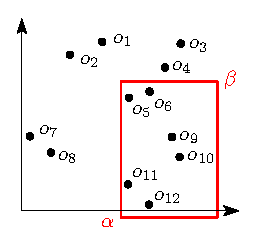
\includegraphics[width=.7\linewidth]{figs/aggregate-queries/example-object.eps}
    \caption{Objects}\label{fig:aggregate-queries:example:object}
  \end{subfigure}~%
  \begin{subfigure}[b]{.5\linewidth}
    \centering
    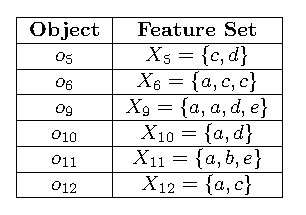
\includegraphics[width=.9\linewidth]{figs/aggregate-queries/example-feature.eps}
    \caption{Features}\label{fig:aggregate-queries:example:feature}
  \end{subfigure}
  \caption{Example of Aggregate Queries}\label{fig:aggregate-queries:example}
\end{figure}

\textbf{Aggregate Queries.} Since the results of aggregate queries are derived from aggregates of data, our study mainly focuses on the following primitive aggregate queries: \emph{max/min}, \emph{count}, \emph{sum}, \emph{top-$k$}, and \emph{frequent feature query (FFQ)}.\footnote{Extension to other more advanced aggregate queries such as \emph{average} and \emph{confidence} will be discussed in \Cref{sec:aggregate-queries:extension}.}  More specifically,  an aggregate query can be expressed in the form of $Q = (q, \{x_i\}, [\alpha, \beta])$, where $q$ is the aggregate operator, $\{x_i\}$ is the queried feature (which is only needed for \emph{count} and \emph{sum}), and $[\alpha, \beta]$ specifies the selection range on the non-sensitive attributes. Consider a sample query $Q = (q, \{x_i\}, [\alpha, \beta])$ in \Cref{fig:aggregate-queries:example}. The query range $[\alpha, \beta]$ selects the objects $o_5, o_6, o_9, o_{10}, o_{11}, o_{12}$. Since $X _5 \uplus X_6 \uplus X_9 \uplus X_{10} \uplus X_{11} \uplus X_{12} = \{(a, 6), (b, 1), (c, 4), (d, 3), (e, 2)\}$, the query result is based on the aggregate operator $q$, as follows:
\begin{itemize}
  \item $q=sum$ or $count$: This sums or counts the multiplicities of $\{x_i\}$ in all selected objects. Supposing $\{x_i\} = \{a\}$, the $sum$ and $count$ results are $(a, 6)$ and $(a, 4)$, respectively.\footnote{The $sum$ and $count$ results will be the same if there are no duplicate elements in the feature sets.}
  \item $q=max$ or $min$: This selects the feature with the maximum or minimum summed multiplicity in all selected objects. If $q=max$, the result is $(a, 6)$; if $q=min$, the result is $(b, 1)$. % chktex 35
  \item $q=$ \emph{top-$k$}: This selects the top-$k$ features with the largest summed multiplicities in all selected objects. Supposing $k$ = 3, the result is $(a, 6), (c, 4), (d, 3)$.
  \item $q=$ \emph{FFQ$_\delta$}: This selects the features whose summed multiplicities in all selected objects are no less than a threshold $\delta$. Supposing $\delta$ = 4, the result is $(a, 6), (c, 4)$.
\end{itemize}

The aggregate queries in \Cref{example:intro:pgp} can be reduced to the above aggregate queries as follows. \textbf{Q1} is simply a $max$ query, i.e., $(max, -, [95014, 95014])$. \textbf{Q2} is a \emph{count} query, i.e., $(count, \{\text{R-G1886S}\}, [00000, 99999])$. \textbf{Q3} is an FFQ query, $(FFQ_3, -, [20000, 29999])$, which finds the set of genes whose sum result is no less than 3. % chktex 35

\textbf{Threat Model and Problem Statement.} We consider two potential security threats:
\begin{inlineenum}
\item the SP could provide unfaithful query execution, thereby returning incorrect or incomplete query results; and
\item data privacy could be breached if sensitive source data are disclosed to the query client.
\end{inlineenum}
Thus, the authentication problem we are investigating is for the query client to verify that the SP executes $Q$ faithfully in terms of the following conditions:
\begin{inlineenum}
\item the candidate objects are correctly selected and no objects in the selection range are skipped;
\item the returned features and multiplicities are not tampered with; and
\item the query result satisfies the aggregation semantics.
\end{inlineenum}
The confidentiality requirement in this problem is to protect the objects' (sensitive) feature sets against the query client. That is, the client cannot infer the features (as well as their multiplicities) of any single object beyond what is implied from the query result.

If neither efficiency nor confidentiality is a concern, authenticating an aggregate query can work as follows. The SP returns a VO to the client, along with the query result. As a naive solution, the VO may include the non-sensitive attributes and sensitive features of all objects in $\mathbb{D}$ and a signature of $\mathbb{D}$. The client uses the VO to verify the soundness and completeness of the results by testing the following conditions:
\begin{itemize}
  \item None of the objects in $\mathbb{D}$ is tampered with.
  \item All candidate objects are in $[\alpha, \beta]$ and no objects in $[\alpha, \beta]$ are missing.
  \item The features and multiplicities of the candidate objects are correct.
  \item The result  satisfies the aggregation semantics of $q$.
\end{itemize}

However, the verification cost of this naive solution is prohibitively high because the entire dataset has to be returned. Moreover, verifying the last two conditions without disclosing sensitive feature sets requires privacy-preserving protocols. To address these issues, we propose an efficient privacy-preserving authentication framework based on verifiable multiset operations, the preliminaries of which are introduced in the next section.

\section{Preliminaries}\label{sec:aggregate-queries:prelim}

This section gives some preliminaries on cryptographic constructs and integrity assurance.

\textbf{Cryptographic Hash Function.}
A cryptographic hash function $H(\cdot)$ accepts an arbitrary-length string as its input and returns a fixed-length bit string. It is collision resistant, i.e., it is difficult to find two different messages $m_1$ and $m_2$ such that $H(m_1) = H(m_2)$. Classic cryptographic hash functions include SHA-1, SHA-2, and SHA-3.

\textbf{Bilinear-Map (BM) Accumulator.} This maps a multiset to a single value for ease of processing. Let $\mathbb{G}$ be a cyclic multiplicative group of order $p$. A BM accumulator is a function of a multiset $X$ of $n$ elements in the cyclic group $\mathbb{Z}_p$~\cite{10.1007/978-3-540-30574-3_19}. It returns an \emph{accumulative value} of $X$:
\begin{align}
  acc(X) = g^{P(X)} = g^{\prod_{x\in{X}}{(x+s)}},
\end{align}
where $g$ is a group generator of $\mathbb{G}$, $s \in \mathbb{Z}_p^* = \mathbb{Z}_p\backslash\{0\}$ is a random secret, and $P(X) = \prod_{x\in{X}}{(x+s)}$.

One useful property of $acc(X)$ is that even without knowing $s$, $acc(X)$ can still be computed by $X$ and $g, g^s, \dots, g^{s^k}$ ($k \ge |X|$) through polynomial interpolation. As for its security, it has been proved in~\cite{10.1007/s00453-014-9968-3} that the accumulative function $acc(\cdot)$ is collision resistant.

\textbf{Randomized BM Accumulator.} The above accumulative value $acc(X)$ is deterministic for a fixed multiset $X$. As such, an adversary can determine with high confidence that two multisets are the same if they happen to have the same accumulative value. To enhance confidentiality, we propose  randomizing the $acc$ value of $X$ as
\begin{align}
  acc(X) = g^{P(X) \cdot r_X},\label{eqn:aggregate-queries:random-bm}
\end{align}
where $r_X$ is a random value hidden from the query client but disclosed to the SP\@. It is worth noting that this randomization does not affect the original properties of a BM accumulator. We will further prove in \Cref{sec:aggregate-queries:security-analysis} that the randomized $acc$ values are indistinguishable under chosen plaintext attack.

\textbf{Bilinear Pairing.} This maps a pair of elements in two groups to a single element in a third group. Let $\mathbb{G}_{t}$ be another cyclic multiplicative group with the same order $p$. We can find a bilinear mapping $e: \mathbb{G} \times \mathbb{G} \rightarrow \mathbb{G}_t$ which has the following properties:
\begin{enumerate}
  \item \emph{Bilinearity}: If $u, v \in \mathbb{G}$ and $e(u,v)\in\mathbb{G}_t$, then $e(u^{a}, v^{b}) = e{(u, v)}^{ab}$ for any $u,v$.
  \item \emph{Non-degeneracy}: $e(g, g) \neq 1$.
  \item \emph{Computability}: Given $u,v\in \mathbb{G}$, it is easy to compute $e(u, v)$.
\end{enumerate}

\textbf{Bilinear $q$-Strong Diffie-Hellman (DH) Assumption.} This assumption shows that bilinear pairing is appropriate for multiset operation authentication as it is hard to forge. Let $(\mathbb{G}, \mathbb{G}_t, e, g)$ be a bilinear pairing. This assumption says that as long as $s\in \mathbb{Z}_p^*$ is secret, even given all elements $g, g^s, \dots, g^{s^k} \in \mathbb{G}$, no probabilistic polynomial-time (PPT) algorithm can derive ${e(g,g)}^{1/(x+s)}$ for any $x\in \mathbb{Z}_p^*$ with a probability higher than a negligible value~\cite{10.1007/978-3-540-28628-8_3}. In essence, this bilinear $q$-strong DH assumption extends the regular DH assumption on $g$ and $\mathbb{G}$ to $e(g,g)$ and $\mathbb{G}_t$. This assumption will be used as a foundation in our security analysis.

\textbf{Set Operation Authentication.} Based on the above, two result verification protocols have been introduced in~\cite{10.1007/978-3-642-54631-0_7,10.1007/978-3-642-22792-9_6} to authenticate the following operations on two sets $X_1$ and $X_2$:
\begin{inlineenum}
\item $X_1 \subseteq X_2$ and~\label{enum:aggregate-queries:prelim:set1}
\item $X_1 \cap X_2 = \emptyset$.~\label{enum:aggregate-queries:prelim:set2}
\end{inlineenum}

For~\ref{enum:aggregate-queries:prelim:set1}, the server computes a witness value $W = acc(X_2 - X_1)$ and returns it to the query client. The client then verifies $X_1 \subseteq X_2$ by checking:
\begin{align*}
  e(acc(X_1), W) \stackrel{?}{=} e(acc(X_2), g).
\end{align*}

For~\ref{enum:aggregate-queries:prelim:set2}, according to the extended Euclidean algorithm, there are two polynomials $Q_1, Q_2$ such that
\begin{align*}
  Q_1 \cdot P(X_1) + Q_2 \cdot P(X_2) = 1.
\end{align*}
As such, the server prepares $F_1 = g^{Q_1}, F_2 = g^{Q_2}$, and then the client verifies it by checking:
\begin{align*}
  e(F_1, acc(X_1)) \cdot e(F_2, acc(X_2)) \stackrel{?}{=} e(g,g).
\end{align*}
Though these two protocols are privacy-preserving in nature and can be extended to multisets, we have yet to design privacy-preserving authentication protocols for other multiset operations such as \emph{sum} and \emph{union}, which will be covered in \Cref{sec:aggregate-queries:multiset-op}.

\section{PA$^2$: Privacy-Preserving Authentication Framework for Aggregate Queries}\label{sec:aggregate-queries:pa2}

\begin{figure}[t]
  \centering
  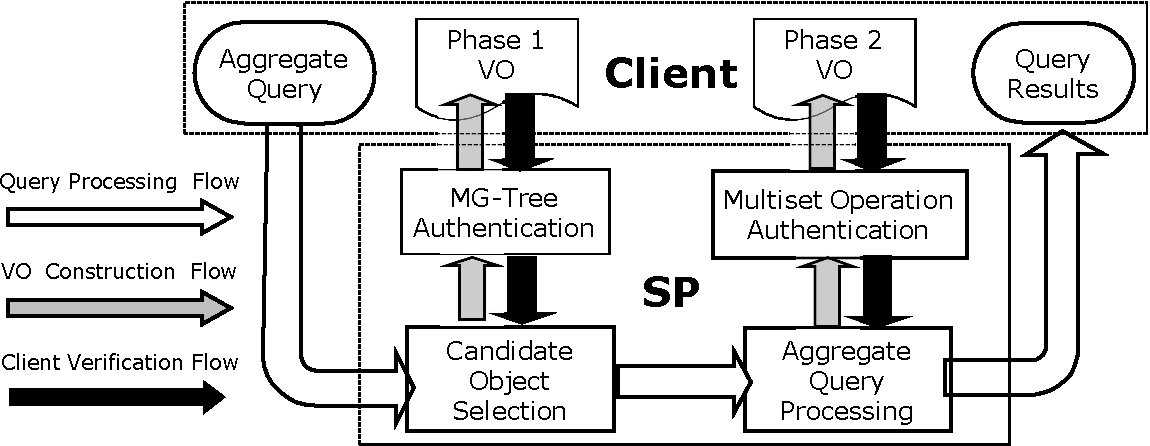
\includegraphics[width=.8\linewidth]{figs/aggregate-queries/overview.pdf}
  \caption{PA$^2$ Authentication Framework Overview}\label{fig:aggregate-queries:overview}
\end{figure}

In this section, we present the complete framework that can authenticate various aggregate queries while preserving data confidentiality. \Cref{fig:aggregate-queries:overview} illustrates both the query and authentication flow charts of the framework. The framework consists of two phases: candidate object selection and aggregate query processing. Recall that given an aggregate query $Q = (q, \{x_i\}, [\alpha, \beta])$, the SP first selects the candidate objects within the range $[\alpha, \beta]$, and then computes the aggregate values of these candidate objects with regard to the queried feature $x_i$. Along with query processing, the SP also constructs the VOs for both phases. Once the client receives the query results and VOs, it can authenticate the correctness of the entire query following the verification flow, which is the opposite of the SP's VO construction flow. In what follows, we present the detailed procedure of each phase in this framework, starting with the second phase for clarity reasons.

\subsection{Privacy-Preserving Authentication Protocols on Multiset Operations}\label{sec:aggregate-queries:multiset-op}

Before running into the detailed procedure of authenticating aggregate queries, we present five core privacy-preserving authentication protocols on multiset operations. The challenge is that the client cannot learn any sensitive feature information when authenticating the multiset operations. Inspired by~\cite{10.1145/2660267.2660373}, our key idea is to leverage the randomized bilinear-map accumulator $acc(\cdot)$ (i.e., \Cref{eqn:aggregate-queries:random-bm}) introduced in \Cref{sec:aggregate-queries:prelim} to hash a multiset into a fixed-length value with collision resistance. With the bilinear pairing function $e(\cdot,\cdot)$ (also introduced in \Cref{sec:aggregate-queries:prelim}), the client can verify the accumulated value of the output multiset without learning the content of each input multiset. This distinguishes the accumulator function from other cryptographic hash functions such as SHA-1.

In the rest of this section, we introduce the five core privacy-preserving authentication protocols on multiset operations, namely, $subset$, $sum$, $empty$, $union$, and $times$. For ease of presentation, we mark below any unverified value computed by the SP with $^*$, while all other unmarked values are trusted or already verified by the candidate object selection protocol (to be explained in \Cref{sec:aggregate-queries:grid}). We also assume that the seeds $g, g^s, \dots, g^{s^k}$ are public and that the random values $r_{X_i}$'s are known to the DO and SP but hidden from the client.

\textbf{Subset:} $sub(X_i, X_j)$.
Given two multisets $X_i, X_j$, it returns the accumulative value $acc(X_j-X_i)$. Note that if $X_i \nsubseteq X_j$, the SP cannot compute a correct value of $acc(X_j - X_i)$. Hence, if $acc(X_j-X_i)$ is verified as correct, the client is assured that $X_i \subseteq X_j$. The detailed protocol is as follows:
\begin{enumerate}
  \item The SP computes the accumulative value ${acc(X_j-X_i)}^*$ based on $X_i$, $X_j$, the random values $r_{X_i}$, $r_{X_j}$, and the public seeds $g, g^s, \dots, g^{s^k}$ (thanks to the nice property of $acc$ as mentioned in \Cref{sec:aggregate-queries:prelim}), and sends it to the client together with $acc(X_i)$ and $acc(X_j)$.
  \item The client verifies the correctness of ${acc(X_j-X_i)}^*$ by checking the following condition, where we exploit the property of bilinear pairing function  $e(\cdot,\cdot)$ as mentioned in \Cref{sec:aggregate-queries:prelim}.
    \begin{align*}
      e(acc(X_i), {acc(X_j-X_i)}^*) \stackrel{?}{=} e(acc(X_j), g).
    \end{align*}
\end{enumerate}

\textbf{Sum:} $sum(\{X_1, \dots, X_n\})$.
Given a set of multisets $\{X_1, \dots, X_n\}$, it returns the accumulative value $acc(S)$ of the sum set $S = \uplus \{X_i\}$. The detailed protocol is as follows:
\begin{enumerate}
  \item The SP computes the accumulative values ${acc(X_1 \uplus X_2)}^*$, ${acc(X_1 \uplus X_2 \uplus X_3)}^*$, $\dots$, ${acc(S)}^*$, and sends them to the client together with $acc(X_1)$, $\dots$, $acc(X_n)$.
  \item The client verifies the correctness of ${acc(S)}^*$ by checking the following equations one by one:
    \begin{align*}
      \left \{
        \begin{array}{l}
          e(acc(X_1), acc(X_2)) \stackrel{?}{=} e({acc(X_1 \uplus X_2)}^*, g)\\
          e({acc(X_1\uplus X_2)}^*, acc(X_3)) \stackrel{?}{=} e({acc(X_1\uplus X_2\uplus X_3)}^*, g) \\
          \vdots\\
          e({acc(\uplus_{i=1}^{n-1} X_i)}^*, acc(X_n)) \stackrel{?}{=} e({acc(S)}^*, g)
        \end{array}
      \right.
    \end{align*}
\end{enumerate}

\textbf{Empty:} $empty(\{X_1, \dots, X_n\})$.
Given a set of multisets $\{X_1, \dots, X_n\}$, it verifies whether $\cap \{X_i\} = \emptyset$. According to the extended Euclidean algorithm, if $\cap \{X_i\} = \emptyset$, there exist $n$ polynomials $Q_i$ such that $\sum_{i=1}^n Q_i \cdot P(X_i) = 1$. The detailed protocol is as follows:
\begin{enumerate}
  \item The SP computes $n$ values $F_i^* = g^{{Q_i}/{r_{X_i}}}$, and sends $F_1^*$, $\dots$, $F_n^*$, $acc(X_1)$, $\dots$, $acc(X_n)$ to the client.
  \item The client verifies the result is empty if the following equation holds:
    \begin{align*}
      \prod_{i=1}^n e(acc(X_i), F_i^*) \stackrel{?}{=} e(g, g).
    \end{align*}
\end{enumerate}

\textbf{Union:} $union(\{X_1, \dots, X_n\})$.
Given a set of multisets $\{X_1, \dots, X_n\}$, it returns the accumulative value $acc(U)$ of the union set $U = \cup_{i=1}^n X_i$. This operation is more complicated than the \emph{sum} operation. Denote $\widehat{X}_i$ as the set version of a multiset $X_i$. The client needs to verify two conditions:
\begin{enumerate}
  \item Deflation checking: $\widehat{X}_1 \subseteq U \wedge \widehat{X}_2 \subseteq U \wedge \cdots \widehat{X}_n \subseteq U$. This is to prevent the SP from deliberately missing any object;
  \item Inflation checking:$(U - \widehat{X}_1) \cap (U - \widehat{X}_2) \cap \cdots (U - \widehat{X}_n) = \emptyset$. This is to prevent the SP from deliberately adding any non-result object.
\end{enumerate}
We can authenticate them based on the above $sub$ and $empty$ protocols as follows:
\begin{enumerate}
  \item Use protocols $sub(\widehat{X}_1, U)$, $sub(\widehat{X}_2, U), \dots, sub(\widehat{X}_n, U)$ to verify the first condition. This not only authenticates $\widehat{X}_i \subseteq U$, but also provides the client the correct $acc(U-\widehat{X}_i)$.
  \item The SP computes a special hash value ${h_e(U)}^*$ of the union set $U$, and by verifying this value the client is assured that the SP knows the pre-image $U$ besides ${acc(U)}^*$.\label{enum:aggregate-queries:multiset-op:union:step2}
  \item Use protocol $empty(\{(U-\widehat{X}_1), (U-\widehat{X}_2), \dots, (U -\widehat{X}_n)\})$ to verify the second condition.
\end{enumerate}
In step~\ref{enum:aggregate-queries:multiset-op:union:step2}, $h_e(\cdot)$ is an \emph{extractable collision resistant hash} (ECRH) function that has one unique property --- extractability~\cite{10.1145/2090236.2090263}. By presenting a correct ${h_e(U)}^*$ value, the SP can prove that it knows $U$. Inspired by~\cite{10.1145/2090236.2090263}, we design $h_e(\cdot)$ for a multiset $X=\{x_1, x_2, \dots, x_t\}$ as follows:
\begin{align*}
  h_e(X) = (h_1, h_2) = (\prod_{i \in [t]} g^{s^i a_i}, \prod_{i \in [t]} g^{\alpha s^i a_i}),
\end{align*}
where $s, \alpha \in \mathbb{Z}_p^*$ are secret values only known to the DO of $X$, and $a_i$ is the $i^{th}$ coefficient for polynomial $P(X)\cdot r_X$. Before any other party can compute or verify $h_e(X)$, the DO releases $g, g^s, \dots, g^{s^k}, g^\alpha, g^{\alpha s}, \dots, g^{\alpha s^k} \in \mathbb{G}$ to the public, where $k \ge |X|$, the cardinality of $X$. Then any party, including the client, can verify whether a hash value $h_e(X)$ is correct by checking the following equations:
\begin{align*}
  e(h_e(X).h_1, g^\alpha) &\stackrel{?}{=} e(h_e(X).h_2, g), \\
  h_e(X).h_1 & \stackrel{?}{=} acc(X).
\end{align*}

\textbf{Times:} $times(X, t)$.
Given a multiset $X$ and a coefficient $t$, it returns the accumulative value $acc(t \cdot X)$ of $t \cdot X$, which raises the multiplicity of each element in $X$ by $t$. For example, if $X = \{(a, 2), (b, 3)\}$, then $3\cdot X = \{(a, 6), (b, 9)\}$. A straightforward solution is to use the $sum$ protocol directly as $sum(\{\overbrace{X, X, \dots, X}^{t}\})$. Here we give a more efficient solution using $sum$ on the binary components. Let $t = {(b_0b_1\cdots b_d)}_2$, the binary form of $t$. The client only needs to execute $sum(\{b_0 \cdot X, \dots, b_i \cdot 2^i \cdot X, \dots, b_d \cdot 2^d \cdot X\})$, where $b_i=1$. For instance, if $t = 5={(101)}_2$, then the client only executes $sum(\{X, 4\cdot X\})$. The detailed protocol is as follows:
\begin{enumerate}
  \item Let $d = \lfloor \log_2(t) \rfloor$, the SP computes ${acc(2\cdot X)}^*, \dots, {acc({2^d} \cdot X)}^*, {acc(t \cdot X)}^*$, and sends them to the client together with $acc(X)$.
  \item The client first verifies the values ${acc(2\cdot X)}^*, \dots, {acc({2^d} \cdot X)}^*$ by checking the following equations:
    \begin{align*}
      \left \{
        \begin{array}{l}
          e(acc(X), acc(X)) \stackrel{?}{=} e({acc(2\cdot X)}^*, g)\\
          e({acc(2\cdot X)}^*, {acc(2\cdot X)}^*) \stackrel{?}{=} e({acc(4 \cdot X)}^*, g) \\
          \vdots\\
          e({acc(2^{d-1} \cdot X)}^*, {acc(2^{d-1} \cdot X)}^*) \stackrel{?}{=} e({acc({2^d} \cdot X)}^*, g)
        \end{array}
      \right.
    \end{align*}
  \item The client then verifies ${acc(t \cdot X)}^*$ according to the binary form of $t(b_0b_1\cdots b_d)$.
\end{enumerate}

We will show in the cost analysis that this protocol significantly improves the performance over the straightforward $sum$ solution.

\subsection{Privacy-Preserving Authentication Algorithms on Aggregate Queries}

Next, we present the detailed procedures of the second phase, i.e., authenticating aggregate queries while preserving data confidentiality. Here, we assume that the output from the first phase of candidate object selection has been verified (to be explained in \Cref{sec:aggregate-queries:grid}). In what follows, $\{X_1, \dots, X_m\}$ are the feature sets of $m$ candidate objects, and $S = \uplus \{X_i\}$ is the sum set. We first study the \emph{sum}/\emph{count} and \emph{max}/\emph{min}/\emph{FFQ}/\emph{top-$k$} aggregate queries and then extend them to other more advanced aggregate queries.

\subsubsection{Sum/Count Query}

The output of a $sum$ query $sum(x_q)$ is $\eta_q$, the sum of multiplicities of feature $x_q$ in all candidate objects. To align with other multiset queries, we define its result as $R = \{(x_q, \eta_q) \}$. For example, in \Cref{fig:aggregate-queries:example}, after selecting the candidate objects $\{o_5, o_6, o_9, $ $\cdots, o_{12}\}$, the query $Q = (sum, \{a\}, [\alpha, \beta])$ returns the sum of multiplicities of feature $a$, i.e., $R = \{(a, 6)\}$.

To verify this result $R$, we design \Cref{alg:aggregate-queries:sum} for the client to check the following two conditions:
\begin{itemize}
  \item Inflation checking (\Crefrange{alg:aggregate-queries:sum:1}{alg:aggregate-queries:sum:3}): $R \subseteq S$. This is to prevent the SP from deliberately increasing the multiplicity of the result;
  \item Deflation checking (\Cref{alg:aggregate-queries:sum:4}): $(S-R) \cap R = \emptyset$. This is to prevent the SP from deliberately decreasing the multiplicity of the result.
\end{itemize}

\begin{algorithm}[t]
  \caption{PA$^2$ Sum ($\{R, X_1, \dots, X_m\}$)}\label{alg:aggregate-queries:sum}
  Obtain $R, acc(X_1), \dots, acc(X_m)$ from the SP (these $acc$ values are authenticated by the MG-tree, to be detailed in \Cref{sec:aggregate-queries:grid}) and compute $acc(R)$ locally\;%
  \label{alg:aggregate-queries:sum:1}
  Execute $sum(\{X_1, \dots, X_m\})$ to get verified $acc(S)$\;%
  \label{alg:aggregate-queries:sum:2}
  Execute $sub(R, S)$ to get verified $acc(S - R)$\tcp*{implies $R \subseteq S$}%
  \label{alg:aggregate-queries:sum:3}
  Execute $empty(S-R, R)$ to verify $(S - R) \cap R = \emptyset$\;%
  \label{alg:aggregate-queries:sum:4}
\end{algorithm}

In the running example, the sum set of the candidate objects' features is $S= \{(a,6)$, $(b, 1)$, $(c, 4)$, $(d, 3)$, $(e, 2)\}$. So the client needs to perform:
\begin{itemize}
  \item Inflation checking: $\{(a, 6)\} \subseteq \{(a,6)$, $(b, 1)$, $(c, 4)$, $(d, 3)$, $(e, 2)\}$;
  \item Deflation checking: $\{(b, 1), (c, 4), (d, 3), (e, 2)\} \cap \{(a, 6)\} = \emptyset$.
\end{itemize}

Similarly, the output of a $count$ query $count(x_q)$ is the number of the candidate objects that have the query feature $x_q$. It can be processed similarly to the $sum$ query, except that the multiplicity of each feature is enforced as $1$.

\subsubsection{Max/Min/FFQ/Top-$k$ Query}

The output of a $max$ query is the feature with the highest (i.e., top-$1$) multiplicity. Let $\tau$ denote this multiplicity, and thus the query is equivalent to searching for any feature whose multiplicity is no less than $\tau$. Formally, the query result  $R = \pi(\{(x_i, \eta_i) | x_i \in S \wedge \eta_i \ge \tau\})$, where $\pi(\cdot)$ randomly selects one feature when there are ties. For example, in \Cref{fig:aggregate-queries:example}, the query $Q=(max, -, [\alpha, \beta])$ returns the result $R = \{(a, 6)\}$. To verify this result, we design \Cref{alg:aggregate-queries:max} for the client to check the following three conditions: % chktex 35
\begin{itemize}
  \item Inflation checking (\Crefrange{alg:aggregate-queries:max:1}{alg:aggregate-queries:max:3}): $R \subseteq S$.
  \item Deflation checking (\Cref{alg:aggregate-queries:max:4}): $(S - R) \cap R = \emptyset$.\footnote{\label{fn:aggregate-queries:skip-deflation}In the actual implementation, the deflation check can be omitted for max, FFQ and top-$k$ queries. This is because it is implied by the following completeness check.}
  \item Completeness checking (\Crefrange{alg:aggregate-queries:max:5}{alg:aggregate-queries:max:8}): $(S - R) \subseteq {\tau} \cdot (U - \widehat{R})$, where $\widehat{R}$ is the set version of multiset $R$, e.g., $R = \{(a, 6)\}$ and $\widehat{R} = \{(a, 1)\}$. This is to prevent the SP from deliberately missing any feature whose multiplicity is larger than $\tau$.
\end{itemize}

\begin{algorithm}[t]
  \caption{PA$^2$ Max ($\{R, X_1, \dots, X_m\}$)}\label{alg:aggregate-queries:max}
  Obtain $R, acc(X_1), \dots, acc(X_m)$ from the SP (these $acc$ values are authenticated by the MG-tree, to be detailed in \Cref{sec:aggregate-queries:grid}) and compute $acc(R)$ and $acc(\widehat{R})$ locally\;%
  \label{alg:aggregate-queries:max:1}
  Execute $sum(\{X_1, \dots, X_m\})$ to get verified $acc(S)$\;%
  \label{alg:aggregate-queries:max:2}
  Execute $sub(R, S)$ to get verified $acc(S - R)$ \tcp*{implies $R \subseteq S$}%
  \label{alg:aggregate-queries:max:3}
  Execute $empty(S-R, R)$ to verify $(S - R) \cap R = \emptyset$%
  \hyperlink{fn:aggregate-queries:skip-deflation}{\footnotemark[\getrefnumber{fn:aggregate-queries:skip-deflation}]}\;%
  \label{alg:aggregate-queries:max:4}
  Execute $union(\{X_1, \dots, X_m\})$ to get verified $acc(U)$\;%
  \label{alg:aggregate-queries:max:5}
  Execute $sub(\widehat{R}, U)$ to get verified $acc(U - \widehat{R})$\;%
  \label{alg:aggregate-queries:max:6}
  Execute $times(U-\widehat{R}, \tau)$ to get verified $acc({\tau} \cdot (U - \widehat{R}))$\;%
  \label{alg:aggregate-queries:max:7}
  Execute $sub(S-R, {\tau} \cdot (U - \widehat{R}))$ to verify $(S-R) \subseteq {\tau} \cdot (U-\widehat{R})$\;%
  \label{alg:aggregate-queries:max:8}
\end{algorithm}

In the running example, the sum set is $S = \{(a, 6), (b, 1), (c, 4), (d, 3), (e, 2)\}$ and the union set is $U = \{(a, 1), (b, 1), (c, 1), (d, 1), (e, 1)\}$. So the client needs to perform:
\begin{itemize}
  \item Inflation checking: $\{(a, 6)\}\subseteq \{(a, 6), (b, 1), (c, 4), (d, 3), (e, 2)\}$;
  \item Deflation checking: $\{(b, 1), (c, 4), (d, 3), (e, 2)\} \cap \{(a, 6)\} = \emptyset$;%
    \hyperlink{fn:aggregate-queries:skip-deflation}{\footnotemark[\getrefnumber{fn:aggregate-queries:skip-deflation}]}
  \item Completeness checking: $\{(b, 1), (c, 4), (d, 3), (e, 2)\} \subseteq \{(b, 6), (c, 6), (d, 6), (e, 6)\}$.
\end{itemize}

The $min$ query is similar except that we verify $(S - R) \supseteq {\tau} \cdot (U - \widehat{R})$ in the completeness checking. % chktex 35

The \emph{FFQ} query returns the features whose multiplicities are no lower than a threshold $\delta$. This query is naturally supported as it is a subroutine of the $max$ query (by replacing the threshold $\tau$ with $\delta$ in the completeness checking). % chktex 35

Similarly, the top-$k$ query can be verified by exploiting the routine of $max$ query and replacing the top-$1$ multiplicity $\tau$ with the top-$k^{th}$ multiplicity. % chktex 35

\subsubsection{Extension to Advanced Aggregate Queries}\label{sec:aggregate-queries:extension}

By fusing multiple primitive aggregate queries, we can further extend our algorithms to support more advanced aggregate queries.

\textbf{Average Query}. The \emph{avg} query returns the average multiplicity of a queried feature. Its result can be authenticated with a $sum$ query and a $count$ query.

\textbf{Confidence Query.} The \emph{confidence} query takes two features as input and returns the conditional probability of witnessing the second feature given the first feature. To revisit Example 1, the confidence that gene `R-G1886S' co-exists with gene `C-R102G' is $\frac{2}{4}=50$\%. This query can be decomposed into two \emph{count} queries for authentication, i.e.,  $(count,  \{\text{R-G1886S}\}, [00000, 99999])$ and $(count, \{\text{R-G1886S}, \text{C-R102G}\}, [00000, 99999])$.

\textbf{Lift Query.} The \emph{lift} query is often used to observe the independence between two features. Given two features $x_1$ and $x_2$, it is defined as the ratio of $count(\{x_1, x_2\})$ to $count({x_1}) \cdot count(x_2)$. In the above example, the lift of gene `R-G1886S' and gene `C-R102G' is $\frac{2}{4 \times 3}=\frac{1}{6}$. Similar to the \emph{confidence} query, its result can be authenticated with three \emph{count} queries, i.e., $(count$, $\{\text{R-G1886S}\}$, $[00000, 99999])$, $(count$, $\{\text{C-R102G}\}$, $[00000, 99999])$, and $(count$, $\{\text{R-G1886S}, \text{C-R102G}\}$, $[00000, 99999])$.

It is noteworthy that as authenticating the above advanced aggregate queries is always reduced to authenticating a set of primitive aggregate queries, the results of those primitive queries are needed by the client to complete the verification chain and are thus not kept confidential. Nevertheless, the confidentiality of source data is still preserved by the privacy-preserving authentication algorithms. Finally, we remark that a multi-feature aggregate query can be supported by treating a multi-feature set as a unique (virtual) feature.

\subsection{Privacy-Preserving Authentication on Candidate Object Selection}\label{sec:aggregate-queries:grid}

\begin{figure}[t]
  \centering
  \begin{subfigure}[b]{.5\linewidth}
    \centering
    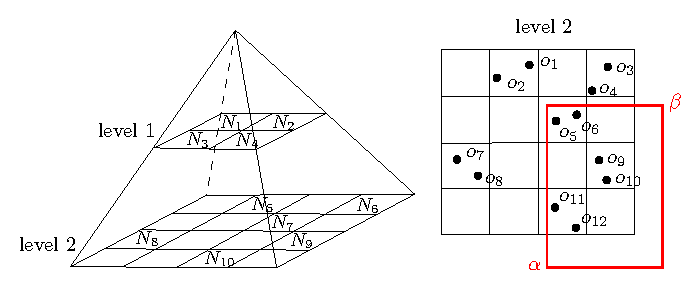
\includegraphics[width=\linewidth]{figs/aggregate-queries/pyramid.eps}
    \caption{Structure}\label{fig:aggregate-queries:mg-tree:structure}
  \end{subfigure}~%
  \begin{subfigure}[b]{0.5\linewidth}
    \centering
    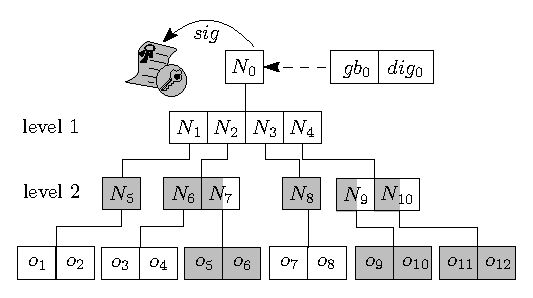
\includegraphics[width=.8\linewidth]{figs/aggregate-queries/grid_tree.eps}
    \caption{Index}\label{fig:aggregate-queries:mg-tree:index}
  \end{subfigure}
  \caption{Merkle Grid Tree (MG-tree)}\label{fig:aggregate-queries:mg-tree}
\end{figure}

Now we turn back to the first phase, i.e., processing and authenticating the candidate object selection. Without loss of generality, we assume that the objects are indexed by a grid structure on their non-sensitive attributes. Thus, we propose \emph{Merkle Grid tree} (MG-tree), an ADS for the DO to construct and sign. Note that our technique can be easily adapted to other multi-dimensional index structures such as R-tree and kd-tree.

\Cref{fig:aggregate-queries:mg-tree:structure} shows a multi-layer grid system, which partitions the space of non-sensitive attributes recursively into multiple levels of grid cells until each cell contains no more than two objects. The bounding box of each cell is called a grid box, and is denoted by $gb$. \Cref{fig:aggregate-queries:mg-tree:index} shows the corresponding MG-tree for the objects in \Cref{fig:aggregate-queries:mg-tree:structure}. Every node $N_i$ corresponds to a non-empty grid cell. Its grid box is denoted by $gb_i$, and has a digest (denoted by $dig_i$) that is computed from its $C$ child entries, $c_1, \dots, c_C$, as follows:

\begin{definition}[Digest for Non-Leaf Node]
  Let $H(\cdot)$ be a cryptographic hash function and `$|$' denote string concatenation. The digest of a non-leaf node is defined as:
  \begin{align*}
    dig_i = H(gb_{c_1} | dig_{c_1} | \cdots | gb_{c_C} | dig_{c_C} ).
  \end{align*}
\end{definition}
For example, in \Cref{fig:aggregate-queries:mg-tree:index}, the digest of node $N_2$, $dig_2 = H(gb_6 | dig_6$ $| gb_7 | dig_7)$.

Now we define the digest of a leaf node based on the $acc$ values of leaf entries.
\begin{definition}[Digest for Leaf Node]
  The digest of a leaf node is defined as:\footnote{In fact, the digest also includes $H(acc(\widehat{X}_{c_1}))|\cdots|H(acc(\widehat{X}_{c_C}))$, where $\widehat{X}_{c_i}$ is the set version of a multiset $X_{c_i}$. These $acc$ values are needed for the $union(\cdot)$ protocol in \Cref{sec:aggregate-queries:multiset-op} but omitted for clarify of presentation.}
  \begin{align*}
    dig_i = H(H(acc(X_{c_1})) | \cdots | H(acc(X_{c_C})) ),
  \end{align*}
  where $acc(X_i)$ is the accumulative value of the feature set of object $X_i$ (defined in \Cref{eqn:aggregate-queries:random-bm}).
\end{definition}
For example, for leaf node $N_5$, its digest ${dig}_5 = H(H(acc(X_1)) | H(acc(X_2)))$. Note that this digest does not need any information about objects' non-sensitive attributes $A_i$, because the digest of its parent node already proves that this object is in its grid box.\footnote{For simplicity, in this paper we assume that the query range aligns with the grid boxes. Otherwise, the definition can be easily extended to include $A_i$ in the digests of leaf nodes.} With these definitions, the DO can compute the $acc$ values of all feature sets and the digests of all nodes in the MG-tree recursively in a bottom-up fashion. The digest of the root entry $dig_0$ is signed by the DO as $sig(dig_0)$.

On the SP side, the processing of a range query $[\alpha, \beta]$ starts from the root node. If a non-leaf node intersects the query range $[\alpha, \beta]$, it will be branched, i.e., its subtree is further explored. On the other hand, if a leaf node intersects the query range $[\alpha, \beta]$, all its entries will be returned as query results. \Cref{fig:aggregate-queries:mg-tree:structure} illustrates an example where $N_0, N_1, \dots, N_{10}$ are nodes and $o_1, o_2, \dots, o_{12}$ are objects, i.e., leaf entries. Since the root node $N_0$ intersects with the range $[\alpha, \beta]$, it will be branched and then non-leaf nodes $N_2, N_4$ are also branched. After that, leaf nodes $N_7, N_{9}, N_{10}$ intersect the query range, and all the leaf entries $\{o_5, o_6, o_{9}, o_{10}, o_{11}, o_{12}\}$ are returned as results, i.e., the selected candidate objects for the next phase of aggregate query processing.

To guarantee the correctness of the selected candidate objects, the query authentication protocol on the MG-tree is as follows:
\begin{itemize}
  \item The SP prepares a VO and sends it to the client. The VO includes:
    \begin{inlineenum}
    \item the grid boxes of all intersected leaf nodes and the accumulative $acc$ values of their leaf entries;
    \item the grid boxes and the digests of all other visited (but not intersected by the query) nodes;
    \item the signature of the root's digest.
    \end{inlineenum}
    For example, in \Cref{fig:aggregate-queries:mg-tree:index}, the VO (marked as grey) includes $\{gb_5$, $dig_5$, $gb_6$, $dig_6$, $gb_7$, $acc(X_5)$, $acc(X_6)$, $gb_8$, $dig_8$, $gb_{9}$, $acc(X_9)$, $acc(X_{10})$, $gb_{10}$, $acc(X_{11})$, $acc(X_{12})$, $sig(dig_0)\}$.
  \item The client first verifies the correctness of the returned results, that is, the grid boxes of all the result nodes are intersected with the query range while all the others are not. Then, the client verifies whether all these information is genuine by restoring the root digest. Specifically, the client recursively rebuilds the digests of leaf nodes and non-leaf nodes up to the root level. Finally, the client checks whether the restored digest matches the signature from the DO\@. If so, the client verifies that all the returned information is genuine. For example, in \Cref{fig:aggregate-queries:mg-tree:index}, the client first verifies $gb_7, gb_9, gb_{10}$ are intersected with the query range $[\alpha, \beta]$, while $gb_5, gb_6, gb_8$ are not. Next, the client rebuilds $dig_{7} = H(H(acc(X_5)) | H(acc(X_6)))$, $dig_{9} = H(H(acc(X_9)) | H(acc(X_{10})))$, $dig_{10} = H(H(acc(X_{11})) | H(acc(X_{12})))$, and then $dig_1 = H(gb_5|dig_5)$, $dig_2 = H(gb_6|dig_6|gb_7|dig_7)$, $dig_3 = H(gb_8|dig_8)$, $dig_4 = H(gb_9|dig_9|gb_{10}|dig_{10})$. And finally, the client restores $dig_0 = H(gb_1|dig_1|\cdots|gb_4|dig_4)$ and checks whether it matches $sig^{-1}(dig_0)$.
\end{itemize}

\subsection{Cost Analysis}\label{sec:aggregate-queries:cost}
In this section, we analyze the performance of PA$^2$ framework. Specifically, we derive cost models for the privacy-preserving authentication protocols on multiset operations, the aggregate query authentication algorithms, and the MG-tree, respectively.

\subsubsection{Cost Model for Authentication Protocols on Multiset Operations}

\begin{table}
  \resizebox{\linewidth}{!}{%
    \begin{tabular}{llll}
      \toprule
      \textbf{Operation} & \textbf{SP Time} & \textbf{Client Time} & \textbf{VO Size} \\
      \midrule
      $sub(X_1, X_2)$ & $C_{sub}^{S}=(|X_2| - |X_1|) \cdot \log_2(p) \cdot C_{gp}$ & $C_{sub}^C= C_{e}$ &  $M_{sub} = 3M_{acc}$ \\
      $sum(\{X_1, \dots, X_n\})$ & $C_{sum}^S = \sum_{i=1}^n (i \cdot |X_i|) \cdot \log_2(p) \cdot C_{gp}$ & $C_{sum}^C=n \cdot C_e$ & $M_{sum} = 2n \cdot M_{acc}$ \\
      $empty(\{X_1, \dots, X_n\})$ & $C_{empty}^S = \max_{i=1}^n (|X_i|) \cdot \log_2(p) \cdot C_{gp}$ & $C_{empty}^C=n \cdot C_e$ & $M_{empty} = 2n \cdot M_{acc}$ \\
      $union(\{X_1, \dots, X_n\})$  &
      \tabincell{@{}r@{$\,$}l@{}}{
      $C_{union}^S =$ & $((n + 1) \cdot |U| - \sum_{i=1}^n |\widehat{X}_i|$ \\
                      & $+ \max_{i=1}^n|\widehat{X}_i|) \cdot \log_2(p) \cdot C_{gp}$
                    }
                      & $C_{union}^C = (2n + 1)\cdot C_e$ &  $M_{union} = (5n +1)\cdot M_{acc}$ \\
      $times(X, t)$  & $C_{times}^S = 2t \cdot |X| \cdot \log_2(p) \cdot C_{gp}$ & $C_{times}^C =2 \log_2(t) \cdot C_e$ &  $M_{times} = 2 \log_2(t) \cdot M_{acc}$ \\
      \bottomrule
  \end{tabular}}
  \caption{Cost Models for Multiset Operations}\label{tab:aggregate-queries:cost-model-set}
\end{table}

\Cref{tab:aggregate-queries:cost-model-set} summarizes the time costs for the SP and client, as well as the VO size for the five core privacy-preserving authentication protocols on multiset operations (\Cref{sec:aggregate-queries:multiset-op}). In this table, $n$ is the total number of objects, $t$ is the second operand for $times(\cdot,\cdot)$, $C_{e}$ is the time cost of a bilinear pairing operation, $C_{gp}$ is the time cost of a multiplication operation in cyclic multiplicative group $\mathbb{G}$ with order $p$, $|U|$ is the size of union set, and $M_{acc}$ is the size of an accumulative value.

\subsubsection{Cost Model for Aggregate Query Authentication Algorithms}
Based on the above analysis, we now derive the cost models for various aggregate queries. Let $m$ be the number of candidate objects, $|S|$ be the size of the sum set, $|\widehat{R}|$ be the size of set $\widehat{R}$, $|X_i|$ be the size of the feature set for the $i^{th}$ candidate object, and $\tau$ be the top-$k^{th}$ (top-1 for a \emph{max} query) multiplicity.

\textbf{Count/Sum Aggregate Query.}
The time cost for the SP is:
\begin{align*}
  C_{count}^S &= C_{sum}^S + C_{sub}^S + C_{empty}^S \nonumber \\
              &= ( \sum_{i=1}^m(i \cdot |X_i|) + |S| - |R| \nonumber\\
              &\quad + \max(|S-R|, |R|)) \cdot \log_2(p) \cdot C_{gp}.
\end{align*}

The time cost for the client is:
\begin{align*}
  C_{count}^C &= C_{sum}^C + C_{sub}^C + C_{empty}^C + |R| \cdot \log_2(p) \cdot C_{gp} \nonumber \\
              &= (2m + 1) \cdot C_e  + |R| \cdot \log_2(p) \cdot C_{gp}.
\end{align*}

The VO size, i.e., the communication cost, is:
\begin{align*}
  M_{count} &= M_{sum} + M_{sub} + M_{empty}\nonumber  \\
            & =  (4m + 3) \cdot M_{acc}.
\end{align*}

\textbf{Max/Min/FFQ/Top-$k$ Aggregate Query.}
The time cost for the SP is:
\begin{align*}
  C_{max}^S &= C_{sum}^S + 3 C_{sub}^S + C_{empty}^S + C_{union}^S + C_{times}^S \nonumber \\ % chktex 35
            &=(\sum_{i=1}^m ( i \cdot |X_i|) + (m+2+2\tau)|U| + max(|S-R|, |R|)\nonumber\\ % chktex 35
            &\quad  + max_{i=1}^n|\widehat{X}_i| - (1 + \tau) |\widehat{R}|- \sum_{i=1}^n|\widehat{X}_i|) \cdot \log_2(p) \cdot C_{gp}. % chktex 35
\end{align*}

The time cost for the client is:
\begin{align*}
  C_{max}^C &= C_{sum}^C + 3 C_{sub}^C + C_{empty}^C + C_{union}^C + C_{times}^C \nonumber\\ % chktex 35
            &\quad + (|R| + |\widehat{R}|) \cdot \log_2(p) \cdot C_{gp}\nonumber \\
            &= (3m + 6 + 2\log_2(\tau)) \cdot C_e + (|R| + |\widehat{R}|) \cdot \log_2(p) \cdot C_{gp}.
\end{align*}

The VO size, i.e., the communication cost, is
\begin{align*}
  M_{max} &= M_{sum} + 3 M_{sub} + M_{empty} + M_{union} + M_{times}\nonumber  \\ % chktex 35
          & =  (7m + 14 + 2 \log_2 (\tau)) \cdot M_{acc}.
\end{align*}

A key observation from the above analysis is that both the client time cost and the VO size are determined only by the result set size and are independent of the number of sensitive features.

\subsubsection{Cost Model for Candidate Object Selection}
We next analyze the cost of the candidate object selection. Our analysis starts with the MG-tree size, based on which we derive the VO construction and verification costs for a range selection. Without loss of generality, the data space is a $d$-dimensional unit space ${[0,1]}^d$, and we assume each non-sensitive attribute independently follows a uniform distribution. As such, the MG-tree partitions each dimension equally and the height of the tree can be approximated as $w=\lceil \log_{2^d}(\frac{n}{f})\rceil$, where $n$ is the total number of objects and $f$ is the minimum number of objects in a leaf node.

\textbf{MG-tree size.} Each tree node stores a grid box (represented by two $d$-dimensional corner points) and a digest. As such, the size of a node, in terms of bytes, is:
\begin{align*}
  M_{N} = 2 \cdot d \cdot 4 + M_h,
\end{align*}
where $M_h$ is the size of a hash value.

Besides the tree nodes, the server stores all leaf entries (i.e., objects). Let $M_{acc}$ denote the size of an accumulative value; then the total size of an MG-tree is:
\begin{equation*}
  M_{MG} = 2 \cdot n \cdot M_{acc} +  \sum\nolimits_{i=0}^{w-1} \min(n, 2^{i \cdot d}) \cdot M_{N}.
\end{equation*}

\textbf{Construction cost of VO.} According to~\cite{10.1145/153850.153878}, the probability that two random rectangles $R_1, R_2$ overlap is:
\begin{equation}
  {\Pr}_{overlap}(R_1, R_2)= \prod\nolimits_{j=1}^d(R_1.L_j + R_2.L_j),
  \label{eqn:aggregate-queries:inter_pro}
\end{equation}
where $R_i.L_j$ is the length of $R_i$ in dimension $j$. Since both the MG-tree partition and object distribution are uniform, the lengths of an intermediate entry at level $i$ and a leaf entry are $2^{-i}$ and $\sqrt[d]{k/n}$, respectively. Putting them into \Cref{eqn:aggregate-queries:inter_pro}, the numbers of visited tree nodes $N_n$ and visited leaf entries $N_e$ are:
\begin{align*}
  N_n &= \sum_{i=0}^{w-1} 2^{i\cdot d}\prod_{j=1}^d(2^{-i}+Q.L_j), \\
  N_e &= n\cdot\prod_{j=1}^d(\sqrt[d]{\frac{k}{n}}+Q.L_j),
\end{align*}
respectively. Let $C_{\otimes}$ denote the time cost of accessing a single entry or a single node. The cost of constructing the VO is modeled as:
\begin{equation*}
  C_{pre} = (N_n + N_e) \cdot C_{\otimes}.
\end{equation*}

\textbf{VO size (communication cost).} A VO includes three parts:
\begin{inlineenum}
\item the grid boxes of all intersected leaf nodes and accumulative values of leaf entries, i.e., $\frac{N_e}{k} \cdot 8 \cdot d + N_e \cdot M_{acc}$;
\item the grid boxes and digests of all boundary nodes, i.e., $N_e \cdot w \cdot (2^d - 1)$;
\item the signature of tree root's digest, i.e., $M_{sig}$.
\end{inlineenum}
As such, the communication cost of the VO is:
\begin{equation*}
  M_{VO} = 8d \frac{N_e}{k}  + N_e \cdot M_{acc} + N_e \cdot w (2^d-1) (8d + M_h) +  M_{sig}.
\end{equation*}

\textbf{Client verification time cost.} The client verifies the VO by first reconstructing the MG-tree, and then checks the signature:
\begin{equation*}
  C_{ver} = (N_n + N_e) \cdot C_{h} + C_{sig},
\end{equation*}
where $C_{h}, C_{sig}$ are the time costs of calculating a hash value and verifying a signature, respectively.

\section{Security Analysis}\label{sec:aggregate-queries:security-analysis}

In this section, we perform a security analysis on our PA$^2$ algorithms for aggregate queries.

\subsection{Security of PA$^2$ Algorithms}

The correctness of our PA$^2$ algorithms is defined in the natural way and is omitted. For soundness, it can be formally defined as follows:

\begin{definition}[Soundness]\label{def:aggregate-queries:sound}
  The PA$^2$ authentication algorithms for aggregate queries are sound if for all PPT adversaries, the success probability is negligible in the following experiment:
  \begin{itemize}
    \item The adversary picks a dataset $\mathbb{D}$.
    \item Run the ADS generation on $\mathbb{D}$ and forward to the adversary.
    \item The adversary outputs a query $Q$, a result $R$, and a VO\@.
  \end{itemize}
  We say the adversary succeeds if the VO passes the result verification and $ R \neq Q(\mathbb{D})$.
\end{definition}

We now show that the PA$^2$ authentication algorithms indeed satisfy the desired security requirements.

\begin{restatable}{theorem}{thm:aggregate-queries:sec}
  The PA$^2$ authentication algorithms for aggregate queries guarantee the correctness and soundness of the query results under the bilinear $q$-strong Diffie-Hellman assumption.
\end{restatable}

\begin{proof}
  The theorem is proved by proving the security of each multiset operation: $sub(\cdot,\cdot)$, $empty(\cdot)$, $sum(\cdot)$, $union(\cdot)$, and $times(\cdot,\cdot)$. See \Cref{app:aggregate-queries} for more detailed proofs.
\end{proof}

\subsection{Privacy Guarantee on Sensitive Features}

Next, we analyze the privacy guarantee on the sensitive features in our PA$^2$ framework. Specifically, we show that the accumulative value of a feature set does not disclose any feature information to the client. Formally, it is stated as follows:

\begin{definition}[IND-CPA]\label{def:aggregate-queries:ind}
  The augmented accumulative value $acc(X)$ for a multiset $X$ is indistinguishable if for all PPT adversaries, there exists a negligible probability $neg(q)$, s.t.
  \begin{align*}
    \Pr[& \textsf{Adv} \to \{X_1, X_2 ,st\}; b \to \{0, 1\}; \\
        & acc(X_b) \to c; \textsf{Adv}(st, c) \to b'; b = b'] = \frac{1}{2} + neg(q).
  \end{align*}
\end{definition}

Before showing the indistinguishability of accumulative values,  we start with the following lemma on the group $\mathbb{G}$.

\begin{lemma}
  For any random value $r \leftarrow \mathbb{Z}_p$, $g^r$ has an equal probability of being any element in $\mathbb{G}$ (with an order of $p$). Formally, for any $\hat g \in \mathbb{G}$,
  \begin{align*}
  \Pr[g^r = \hat g] = 1 / p.
  \end{align*}
\end{lemma}
\begin{proof}
  Let $\log_g(\cdot)$ denote the discrete logarithm of base $g$ in group $\mathbb{G}$. We have
  \begin{align*}
  \Pr[g^r = \hat g] = \Pr[r = \log_g(\hat g)].
  \end{align*}
  Since $r$ is random, the probability of $r$ being a fixed element $\log_g(\hat g)$ equals $1/p$.
\end{proof}

Now we show a theorem on the security of accumulative values.
\begin{theorem}\label{thm:aggregate-queries:cpa}
  The augmented accumulative value $acc(X)$ for a multiset $X$ is indistinguishable under chosen plaintext attack (CPA).
\end{theorem}
\begin{proof}
  Since the augmented accumulative value $acc(X)=g^{P(X) \cdot r_X} = {(g ^ {P(X)})}^{r_X}$, according to the above lemma, $acc(X)$ has an equal probability of being any element in $\mathbb{G}$. As such, the verifier learns nothing about $P(X)$ and any element $x_i \in X$. Further, since $r_X$ is random for each $X$, $acc(X)$ is indistinguishable under CPA\@.
\end{proof}

It is worth noting that by achieving indistinguishability on a single accumulative value, multiple accumulative values are automatically guaranteed to be indistinguishable.
Therefore, the above theorem effectively proves the security of the authentication algorithms developed for various primitive aggregate queries, as only (indistinguishable) accumulative values are disclosed for the sensitive features throughout the authentication process, which protects the confidentiality of source data.

\subsection{Discussion on Privacy Guarantee}
It is noteworthy that during the authentication of aggregate queries, the results of primitive aggregate queries are disclosed to the client, which might be a source of privacy leak. In an extreme case, if there is only one candidate object in the selection phase, the query result could directly reveal the features of that object. Further, the difference of two query results could reveal the features of the difference of the two candidate object sets. As more aggregate queries are issued and each may consist of multiple primitive aggregate queries, it becomes easier to find smaller difference of candidate object sets. To mitigate such privacy leak, inspired by the bucketization approach~\cite{ppdp09}, we impose a minimum granularity on the MG-tree leaf nodes for the non-sensitive attributes. Specifically, when building the MG-tree, the DO enforces each leaf node (i.e., a bucket) to contain a minimum number of objects that can satisfy a given privacy metric (e.g., $k$-anonymity or $t$-closeness~\cite{Samarati98, Li2007}). As such, the data space is partitioned into disjoint buckets, and upon query processing, a bucket is the smallest granule for range selection. With this enforcement, no query result can reveal whether it is contributed by a specific object in a bucket, and the latter becomes the smallest granule of result privacy leak, no matter how many aggregate queries are issued. Formally, the results of aggregate queries and the associated authentication process achieve the following \emph{bucket-wise indistinguishability} privacy:
\begin{definition}[Bucket-wise Indistinguishability]\label{def:aggregate-queries:k-anony}
  Given a bucket $\mathcal{B}$ and an object $o\in\mathcal{B}$, if an aggregate query result $R$ is from a candidate object set $\mathcal{O}\supseteq \mathcal{B}$, then any adversary can determine whether $o$ contributes to $R$ with a success rate no higher than that of a random guess.
\end{definition}

